\langueeng

\chapter*{Introduction}

%% Ici j'ai essayé de remplacer par \langueeng mais sans succès du tout! Du coup je commence à remplir avec du texte anglais

This introduction is divided into three parts: (i)~a brief presentation of the language and of the collaborations which made it possible to produce the dictionary (§\ref{sec:lang}), (ii)~a User's Guide (§\ref{sec:guide}), and finally (iii)~some general reflections which aim to explain what is at stake in lexicographical work on endangered languages.


\section{The Yongning Na language}
\label{sec:lang}

The Na (Moso) are famous among anthropologists for their family structures, as a “society without marriage” \parencite{cai1997,wellens2003,milan_tourisme_2019}. Until the 21st century, much less attention was directed to their language, which has fascinating properties, such as its elaborate morphotonology.

This dictionary documents the lexicon of the Yongning Na language, \phonologie{nɑ˩-ʐwɤ˥}, an autonym romanized as ‘Narua’\parencite{dobbs_ortho_2018}. It is known in China as ‘Mosuo’ \pcmn{摩梭话}, and classified as an ‘Eastern dialect’ of the Naxi language \parencite[107]{heetal1985}. The language’s Ethnologue code is \textsc{nru} \parencite{lewisetal2016} and its Glottolog code is \textsc{yong1270} \parencite{Nordhoff2012}. The name ‘Yongning Na’ was coined by Liberty \textcite{lidz2006} by associating the people's {endonym} with the name of the place where the language is spoken:
% Map~\ref{map:1-1} locates this language on a~map of Asia showing the current geographical distribution of \il{Sino-Tibetan}Sino-Tibetan languages.\footnote{Issues of language classification are addressed in \sectref{sec:thepositionofnaandnaxiwithinsinotibetan}.}
the plain of Yongning \pcmn{永宁}, a~basin located in Southwestern China, at the border between Yunnan and Sichuan, at a latitude of 27°50’ N and a longitude of 100°41’ (see map \ref{map:1-1}). Yongning is close to Lugu Lake \pcmn{泸沽湖} (in Na: \phonologie{lo˧ʂv̩˩-hi˩nɑ˧mi˧}), a~lake of about fifty square kilometres which creates a~microclimate that is suitable for farming despite the high altitude (about 2,800 meters above sea level).

\begin{mapfigure}[htp]
	\caption{A sketch map of the Yongning area. \emph{Designed by Jérôme Picard. Sources: Geofabrik, ASTER GDEM (a product of METI and NASA) and OpenStreetMap.}}
	\includegraphics[width=.86\textwidth]{Lien vers images/PDF_CMYK_1point4.pdf}
	\label{map:1-1}
\end{mapfigure}

The total number of speakers was estimated at about 40,000 on the basis of survey data from the late 1950s \parencite[107]{heetal1985}; the same figure is taken up by \parencite{yang2009}. The number of proficient speakers in the 2020s is much lower: language replacement (by Mandarin) is under way.

Since the 1990s, and especially in the 21st century, the Yongning region has become a major tourist destination. An anthropological study of the impacts of this new industry \parencite{milan_tourisme_2019} echoes the intuition of a contemporary poet:

\begin{quote}
    Tourism has spread like floodwaters carrying wrecks. It dislocates even the most remote villages, and trumpets its empty, arrogant formulas in the most secret chambers of temples: stereotypes that are, alas, typical of our Western culture. Advertising brochures are nobody's speech; they tend to force the inhabitants of the places visited to see themselves from the outside, to tell their own stories in the way that lazy visitors wish them to, and to replace their own intuitions and memories by gaudy pictures to cater for the taste of visitors. (Yves Bonnefoy, \emph{L'Inachevable. Entretiens sur la poésie}, 1990-2010. Paris: Albin Michel, 2014, p. 232.)
\end{quote}

This context lends extra significance to the task of paying attention to the language of the Na, at a time when it is being rapidly replaced by Mandarin Chinese (the language of schooling, of the media, and of tourism). I have a hope that the recordings made in the field, and gradually transcribed, translated and annotated, will succeed in preserving and transmitting, in all its freshness, the speech of this volume's co-author, which she has agreed to make public for the sake of research and of posterity. The dictionary is intended as a tool for accessing these documents, which document a disappearing language and culture that have value, not only in the abstract sense of being possible and attested forms of human language and society (to be taken into account in typological models and in historical accounts), but in and of themselves.

	\begin{quote}
    \emph{The world}, to us, (...) is it not first and foremost fields which have been cleared and ploughed by people who were thereby founding, grounding, their presence in a specific place? If it be thus, words would be a way to inscribe and express a sense of presence projected onto a rough `out there' (...). Or let's put it this way: What if words were not means to handle general, abstract notions, but windows onto the relationship established between a human presence and a place? Then words would not serve as a ``lexicon'' of what we call \emph{nature}: they would constitute doors opening onto a land (a `sojourn', as Mallarmé put it) where we can be at home, where familiar names create bounding horizons. If it be so, each and every encounter would be a chunk of our destiny, not an abstract event feeding into some scientific generalizations. Our awakened consciousness should hold onto it as something open and possible (even though the swift course of time robs us of so many of such possibilities). We should not erase living encounters from our speech, dismissing them as mere examples of some abstract, timeless scheme. (Yves Bonnefoy, «La fleur double, la sente étroite: la nuée», reprinted in \emph{La Vérité de parole et autres essais}, Paris: Gallimard, 1995, pp. 566-567).
\end{quote}

\subsection{Bibliographical indications}

Important references on Na include a reference grammar of a dialect close to the one described here: that of Luoshui \pcmn{落水} \parencite{lidz2010}, as well as research into the tone systems of previously undocumented dialects \parencite{a2016,dobbsetal2016,fily_documentation_2022}. Concerning lexicographic work, \emph{An anthology of everyday words and expressions in the Mosuo language} \parencite{zhibaetal2013} presents vocabulary and expressions arranged by semantic field. The authors are a native speaker from the Lake area (\pcmn{泸沽湖}) and a doctor in linguistics from Yunnan University. Their fieldwork is described as covering the Yongning plain and the Lake area, but with the Yongning plain as the main research area (p. 2). Approximations in phonetic notation are so numerous that they make the volume unreliable as a work of reference. Voicing contrasts were challenging for the linguist in the team, whose training was mainly focused on the theory and practice of teaching Chinese as a foreign language. Thus, the name of the mountain \phonologie{kɤ˧mv̩˧˥} is transcribed as \phonétique{gə⁵⁵mu⁵⁵}, with a voiced initial (p. 17 and elsewhere). The mountain’s name in Chinese, \pcmn{格姆山}, \emph{Gemu} in romanized Chinese, may have exerted an influence here. Conversely, the adjective \phonologie{dʑɤ˩} ‘good’ is transcribed as \phonétique{tɕɑ¹³}, with an unvoiced initial. Some phonemes, such as uvulars, are absent from the notations. There is thus clearly a gap to be filled in lexicographic work on Na. Dictionaries on neighbouring Naxi provide a brilliant example to be emulated \parencite{heetal2011,pinsonetal2012}.

\subsection{Dialect and language consultants}

Unless otherwise stated, all the data are from the second author, Mrs.\ Latami Daeshilamu (\phonologie{lɑ˧tʰɑ˧mi˥ ʈæ˧ʂɯ˧-lɑ˩mv̩˩}; Chinese: \pcmn{拉它米打史拉么} Lātāmǐ Dǎshǐlāme). She was born in 1950 in the hamlet called Alawua \phonologie{ə˧lɑ˧-ʁwɤ\#˥}, close to the monastery of Yongning. The administrative coordinates of this hamlet are: Yúnnán province, Lìjiāng municipality, Nínglàng Yí autonomous county, Yǒngníng town, Ālāwǎ village (\pcmn{云南省丽江市宁蒗彝族自治县永宁镇}\footnote{Yongning Township in Ninglang Yi Autonomous County, Lijiang City, Yunnan Province, China (\pcmn{云南省丽江市宁蒗彝族自治县永宁乡}) was renamed Yongning Town \pcmn{永宁镇} on February 11th, 2019.}\pcmn{阿拉瓦村}). This language variety corresponds to the Glottolog code \textsc{yong1288}, as distinct from the Lataddi variety (Lataddi Narua), spoken on the shore of Lugu Lake (code: \textsc{lata1234}).

The choice to work in one location only, and essentially with one consultant, is based on the investigator’s initial focus on the tone system. There is considerable dialectal diversity within the Na area (much more so than in the Naxi-speaking area); the tone systems of different villages are conspicuously different, and this geographical diversity combines with dramatic differences across social groups, and across generations. The obvious thing to do seemed to be an in-depth description and analysis of the language as spoken by one person (simultaneously making a few forays into other idiolects and dialects). The collaboration went well, so much so that Mrs.\ Latami accepted (in 2024) the proposal to have her name appear as coauthor of the present volume.

Data from other speakers are indicated in the dictionary using two-letter initials, provided in the leftmost column in Table \ref{table:ConsultantsTable}. The table indicates the correspondence with the speaker codes in A.\ Michaud's database (such as `F4' for the main consultant and coauthor of this volume). The numbering of Na consultants in terms of these speaker codes is discontinuous (F4, F5, F6, F22 and M18, M21, M23 instead of F1 through F4 and M1 through M3) because they were assigned as part of a list of consultants for all three languages of the Naish group: Naxi, Na and Laze.

\begin{longtblr}[
  caption = {Language consultants},
  label = {table:ConsultantsTable}
]{
  colspec = {X[0.6,l,m]X[1.1,l,m]X[l,m]X[l,m]X[0.6,l,m]X[0.3,l,m]},
  rowhead = 1
}
  \hline
  {initials} & {name in orthography} & {name in phonetic alphabet} & {name in Chinese} & {year of birth} & {speaker code} \\
  \hline
        La & Latami Daeshi Lamu & \phonologiebis{lɑ˧tʰɑ˧mi˥ ʈæ˧ʂɯ˧-lɑ˩mv̩˩} & 拉它米旦史拉么 & 1950 & F4 \\
        Gi & Gisso & \phonologiebis{ki˧zo˧} & 郭给若 & 1973 & F5 \\
        Qi & Qiddeu & \phonologiebis{tɕʰi˧ɖv̩\#˥} & 郭园芝 & 1987 & F6 \\
        Sg & Siggeema & \phonologiebis{sɯ˧gɯ˧mɑ˧} & 思格玛 & 1987 & F22 \\
        Da & Latami Daeshi Daedeu & \phonologiebis{lɑ˧tʰɑ˧mi˥ ʈæ˧ʂɯ˧-ʈæ˩ʈv̩˩} & 拉他咪王勇 & 1972 & M18 \\
        Jj & Ho Jjacee & \phonologiebis{ho˧dʑɤ˧tsʰe˥} & 何甲泽 & 1942 & M21 \\
        Dd & Ddeezzhi  & \phonologiebis{ɖɯ˩ɖʐɯ˧} & 何独知 & 1974 & M23 \\
  \hline
\end{longtblr}

The small circle of consultants has grown organically over time. The first contact was Latami Daeshi (M18), who kindly undertook to look for language consultants in the village. As explained elsewhere \parencite[28-29]{michaud2017}, this search did not prove fruitful at first, and it was his mother (F4) who agreed to take on the role of consultant-teacher. She remains a constant point of reference, the main source for the linguist's work and a daily dialogue partner in the field. Her daughter-in-law (F5) agreed to lend a hand, as did one of the latter's nieces (F6). Later, one of F4's cousins (M21) and his son (M23) also took part in the survey.
Finally, Siggeema (F22) is from the village of Wualabbi; she participates in the project through orthography testing and correction work with Roselle Dobbs, and by providing insider information on various topics of Moso phonetics, semantics, grammar and dialectology.

The small sample that has thus been built up over time, without any fixed overall plan, is not balanced according to any particular criterion, and no claim is made that it is representative in any sense. Nevertheless, some of its characteristics can be noted in retrospect.

In terms of generations, the sample shows a certain diversity. The speakers do not all belong to the same lineage, but belong to three successive generations. F4, co-author of the volume, was born in 1950 and is of the same generation as M21. The next generation is represented by M18 (her son), F5 (her daughter-in-law) and M23 (M21's son). F6 and F22 are younger, so much so that they can be considered as belonging to a third generation.

In terms of relationship to the language and culture:

\begin{itemize}
    \item F4 is the most immersed in Na culture, having resided continuously in Yongning for sixty years (from birth until 2010).
    \item F5 and M23 belong to the next generation of speakers who remained in the village (where they still lived as of 2024), for whom local Chinese (Southwestern Mandarin) is a language spoken fluently from a young age, close to a \emph{second mother tongue}.
    \item M18 has a lifelong commitment to research on the Na culture, to which he has deep attachment. He uses the language on a day-to-day basis with his mother (F4). He expresses himself fluently in Na\footnote{Eight recordings (audio and video) that he has made on the following themes can be consulted online:
    \href{https://doi.org/10.24397/pangloss-0007734}{1: Yongning and the Na}; \href{https://doi.org/10.24397/pangloss-0007740}{2: the ethnonym `Moso': its history and relevance}; \href{https://doi.org/10.24397/pangloss-0007730}{3: personal narrative}; \href{https://doi.org/10.24397/pangloss-0007736}{4} and \href{https://doi.org/10. 24397/pangloss-0007738}{5}: a look back at the collaboration with the linguist-investigator; \href{https://doi.org/10.24397/pangloss-0007742}{6: a review of Moso studies}; \href{https://doi.org/10.24397/pangloss-0007728}{7: the cultural values inherited by young people}; \href{https://doi.org/10.24397/pangloss-0007732}{8: the symbolic importance of the hearth in Moso culture}.}.
    However, the title of \pcmn{心碎与忧伤} (\emph{Grief and sorrow}) that he gave to a collection of his papers \parencite{latami2016} speaks volumes about the tensions inherent in living one's life as a reader, researcher and writer in a language which is not that of one's ``mother culture".
    \item M21 has lived in various places in the region, and the dialectal adjustments made in the course of his life naturally led to a certain distance between his speech and that of speakers with a less diverse experience. We are particularly grateful for his efforts to take part in the work despite his partial deafness.
\end{itemize}

Today, as in the past, a constant goal and hope is to involve speakers as closely as possible in research into their language. The decision to have this book co-authored by the main consultant is in keeping with this logic. Her son Latami Wangyong did not wait for the exchanges with Alexis Michaud to enter the circle of scholars. As an ethnologist specializing in Na culture, his contribution to this book is grounded in his scholarly perspective, rather than in his status as a native speaker.

\subsubsection{Other collaborators}

Other collaborators include:

\begin{itemize}
    \item Roselle Dobbs (Ddeema Lhaco, \pcmn{杜玫瑰}) and her Moso friends and collaborators, to whom I owe, in addition to the spelling with which Roselle has endowed this dictionary, a flow of information, corrections and advice since the beginning of my research into Yongning Na.
    \item Benjamin Galliot, who has been editing the dictionary since 2016 to the highest computational and typographic standards, with an exceptional degree of attention to detail as well as to overall structure.
\end{itemize}

The term \emph{consultant} could also be used for these collaborators, insofar as they provide expert advice, corrections and observations of all kinds as the work progresses. This usage is certainly too paradoxical in the light of current practices (where the term is used for \emph{language consultants}, referred to in the past as \emph{informants}) for us to be tempted to adopt it; however, it would have the advantage of not creating a boundary between two groups: native speakers and others, but on the contrary of emphasizing that the dictionary is the fruit of team work.

\subsubsection{The Alawua speech variety and its dialectal context}

The contours of the \emph{communities} within which the Na dialects are spoken are not necessarily as clearly delineated as in Native American or Aboriginal Australian societies, which constitute an important reference in most contemporary English-language methodological work.\footnote{Thus, the term `community' appears no less than thirty-one times in an article about immersion language fieldwork methods written by a colleague affiliated with the University of Sydney: “Enhancing data collection through linguistic competence in a field language: Perspectives from rural China”. Manuel David González Pérez's article is based on in-depth reflections on fieldwork carried out on a Yi language from Yunnan; close to 200 references are cited, reporting experiences that concern a wide variety of languages, but all are English-language references (with the exception of two in German and two in Spanish), which entails a slight risk of cultural bias. This cultural bias could have consequences comparable to the linguistic bias whereby too few languages are taken into consideration when formulating linguistic generalizations (it has been pointed out that “language research shows a lack of openness to diverse languages and populations”: \cite[23]{bochynska_reproducible_2023}). González Pérez does not mention local (Chinese or Yi) equivalents for the term `community', or specificities in the understanding of group dynamics as they relate to language use: no mention is made of language policies or the political context of present-day China~-- which may seem paradoxical given the observation of other foreign visitors that politics is by no means absent from people's preoccupations in the Middle Kingdom (among many examples, see Henri Michaux, \emph{Un barbare en Asie}, Paris: Gallimard, 1967, pages 178sq). It goes without saying that this remark does not constitute a criticism aimed at the author, who could not possibly go into all and every issue related to the vast topic broached in the article cited. The idea is simply to point out the ever-present risk of being wrapped up in one's own views, forgetting that the socio-geo-political diversity of situations is virtually infinite, and putting forward unwarranted generalizations about situations in the field.}
Moso speakers' sense of belonging is an area that is not only complex (as is natural in human societies) but also politically sensitive, in the context of a contemporary China whose resolutely assimilationist plans aim to melt the former ``minority nationalities" (\pcmn{少数民族}) into the melting-pot of the ``Chinese people" (\pcmn{中华民族}). No attempt will be made here to define the geographical boundaries of a ``Alawua dialect of Na" that would extend beyond this hamlet to cover such and such an area on a dialect map. The label ``speech variety spoken in Alawua" is considered as a sufficient language tag for the corpus collected in this one location: no attempt is made to place this speech variety within a comprehensive list of all Moso dialects.

It could be argued, however, that the mere fact of endowing this speech variety with a dictionary gives it a prominent place in a contemporary lexicographical landscape that is still very sparse. Seen in this light, the orthographic representation provided in the dictionary has special value, as it aims to achieve a certain balance between dialects: it is not based on one dialect only (or have one specific speaker as an authoritative reference).

\subsection{Aims and chronology of the project}

\begin{quotation}
    Adams, our head-boy, who had a turn for mathematics, had made a calculation, I was informed, of the time this Dictionary [a new Dictionary which Dr. Strong, the headmaster, had in contemplation] would take in completing, on the Doctor’s plan, and at the Doctor’s rate of going. He considered that it might be done in one thousand six hundred and forty-nine years, counting from the Doctor’s last, or sixty-second, birthday. (Charles Dickens, \emph{David Copperfield} (1850), Chapter 16.)
\end{quotation}

\begin{quotation}
    Since the project is constrained by limited resources of money, staff and time, the project must be organized in such a way that even after a very short period the dictionary makers can produce a useful piece of work. \parencite[``Dictionary making in endangered speech communities'':][42]{mosel_dictionary_2004}
\end{quotation}

\subsubsection{Elicitation method}

In the classical tradition of linguistic fieldwork, a language description should include a dictionary, a grammar, and a collection of texts. Linguistic fieldwork consists in “going into a community where a language is spoken, collecting data from fluent native speakers, analysing the data, and providing a comprehensive description, consisting of grammar, texts and dictionary” \parencite[12]{dixon2007}. The grammar, texts and dictionary are referred to as the “Boasian trilogy” \parencite{foley1999} by reference to Franz Boas’s foundational work collecting North American languages \parencite{boas1902,boasetal1911}. Thus, the lexicographic data presented in this volume were collected as part of all-out fieldwork on Yongning Na. Trips to the field were made in 2006, 2007, 2008 and 2009, followed in 2011-2012 by a one-year stay in the city of Lijiang, where Ms. Latami Daeshilamu had settled to take care of a grandchild. Shorter stays were made in 2013, 2014, 2018 and 2024.


%xxxx A set of Na recordings with time-aligned transcriptions is available from the Pangloss Collection \parencite{michailovskyetal2014}.\footnote{\url{https://pangloss.cnrs.fr/corpus/Yongning_Na}}
% A book-length study of Na morphotonology \parencite{michaud2017} is available online. It also contains detailed information on the phonemic analysis.

A list of words was begun through elicitation, and gradually expanded and corrected as narratives were recorded and transcribed. A drawback of not eliciting large amounts of vocabulary is that addition of new words is a slow process. Hence the limited number of entries: on the order of 3,000 (the current count stands at \obtenircompteur{total}). On the other hand, an advantage of placing the emphasis on text collection is that a context is available to help clarify the meaning of newly encountered words, also offering a basis for further discussion of their usage with language consultants.

\begin{quotation}
    The native speaker interviewees might feel very embarrassed when they are asked to translate a word they do not understand, or even worse, a word which they cannot translate because they have forgotten the native language equivalent.

Words which have been elicited by translation always need to be counterchecked by translating them later back into English or by explaining their meaning. The meaning of the indigenous word may be broader or narrower than its English counterpart, and the words in either language may be polysemous in different ways so that their meanings only partly overlap. \parencite[44]{mosel_dictionary_2004}
\end{quotation}

The word list as of 2011 was deposited in the Sino-Tibetan Etymological Dictionary and Thesaurus (STEDT) database \parencite{stedt}, at the request of the curators. The same year, under the impetus of Guillaume Jacques and Aimée Lahaussois, plans were made to bring the word list closer to the standards of a full-fledged dictionary. A project was deposited with the \emph{Agence Nationale de la Recherche}, accepted in 2012, and begun in 2013: the HimalCo project (ANR-12-CORP-0006).

Dictionaries constitute work-in-progress. Successive versions are numbered, following the model used in software development. %Major releases are expected to occur at most every few years.
The versions produced so far are presented below in chronological order. A summary in table form is provided in Table \ref{table:versionsEN} for English-language editions. Chinese-language editions are shown in Table \ref{table:versionsZH}, and French-language editions in Table \ref{table:versionsFR}.


\begin{longtblr}[
  caption = {Successive versions of the English-language edition},
  label = {table:versionsEN}
]{
  colspec = {X[0.8,l,m]X[0.8,l,m]X[l,m]X[1.4,l,m]},
  rowhead = 1
}
  \hline
  number & date & link to online deposit & software library \\
  \hline
  1.0 & September 2015 & \href{https://shs.hal.science/halshs-01204638v1/}{halshs-01204638v1} & \href{https://github.com/CNRS-LACITO/HimalCo/tree/master/dev/lib/pylmflib-1.1}{PyLMFlib} \\
  1.1 & November 2016 & \href{https://shs.hal.science/halshs-01204638v2/}{halshs-01204638v2} & \href{https://github.com/CNRS-LACITO/HimalCo/tree/master/dev/lib/pylmflib-1.1}{PyLMFlib} \\
  1.2.1 & April 2018 & \href{https://shs.hal.science/halshs-01204638v3/}{halshs-01204638v3} & \href{https://github.com/CNRS-LACITO/Lexika}{Lexika (language: Python)} \\
  1.2.2 & July 2018 & \emph{no deposit in HAL} & \href{https://github.com/CNRS-LACITO/Lexika}{Lexika (language: Python)} \\
  2.0 & 2024 & \href{https://shs.hal.science/halshs-01204638v4/}{halshs-01204638v4} & \href{https://gitlab.com/BenjaminGalliot/JLexika}{JLexika (language: Julia)} \\
  % \pnrubis{pò-ko-kabu} & \pnrubis{po-ko-kabun} & jeudi (3 j. [avant le] jour sacré) \\
  % \pnrubis{pò-tru kabu} & \pnrubis{po-ru-kabun} & vendredi (2 j. [avant le] jour sacré) \\
  % \pnrubis{po-xè kabu} & \pnrubis{po-xe kabun} & samedi (1 j. [avant le] jour sacré) \\
  \hline
\end{longtblr}

\begin{longtblr}[
  caption = {Successive versions of the Chinese-language edition},
  label = {table:versionsZH}
]{
  colspec = {X[0.8,l,m]X[0.8,l,m]X[l,m]X[1.4,l,m]},
  rowhead = 1
}
  \hline
  number & date & link to online deposit & software library \\
  \hline
  \hline
  1.2 & March 2018 & \href{https://shs.hal.science/halshs-01744420v1/}{halshs-01744420v1} & \href{https://github.com/CNRS-LACITO/Lexika}{Lexika (language: Python)} \\
  2.0 & 2024 & \href{https://shs.hal.science/halshs-01744420v2/}{halshs-01744420v2} & \href{https://gitlab.com/BenjaminGalliot/JLexika}{JLexika (language: Julia)}\\
  \hline
\end{longtblr}

\begin{longtblr}[
  caption = {Successive versions of the French-language edition},
  label = {table:versionsFR}
]{
  colspec = {X[0.8,l,m]X[0.8,l,m]X[l,m]X[1.4,l,m]},
  rowhead = 1
}
  \hline
  number & date & link to online deposit & software library \\
  \hline
  \hline
  1.0 & September 2015 & \href{https://shs.hal.science/halshs-01204645v1/}{halshs-01204645v1} & \href{https://github.com/CNRS-LACITO/HimalCo/tree/master/dev/lib/pylmflib-1.1}{PyLMFlib} \\
  1.1 & November 2016 & \href{https://shs.hal.science/halshs-01204645v2/}{halshs-01204645v2} & \href{https://github.com/CNRS-LACITO/HimalCo/tree/master/dev/lib/pylmflib-1.1}{PyLMFlib} \\
  1.2.1 & April 2018 & \href{https://shs.hal.science/halshs-01204645v3/}{halshs-01204645v3} & \href{https://github.com/CNRS-LACITO/Lexika}{Lexika (language: Python)} \\
  2.0 & 2024 & \href{https://shs.hal.science/halshs-01204645v4/}{halshs-01204645v4} & \href{https://gitlab.com/BenjaminGalliot/JLexika}{JLexika (language: Julia)} \\
  % \pnrubis{pò-ko-kabu} & \pnrubis{po-ko-kabun} & jeudi (3 j. [avant le] jour sacré) \\
  % \pnrubis{pò-tru kabu} & \pnrubis{po-ru-kabun} & vendredi (2 j. [avant le] jour sacré) \\
  % \pnrubis{po-xè kabu} & \pnrubis{po-xe kabun} & samedi (1 j. [avant le] jour sacré) \\
  \hline
\end{longtblr}

% \begin{longtblr}[
%   caption = {Successive versions of the Na-English-Chinese-French dictionary (English-language format)},
%   label = {table:versionsEN}
% ]{
%   colspec = {X[1,l,m]X[l,m]X[2.5,l,m]},
%   rowhead = 1
% }
%   \hline
%   numérotation & date & lien vers HAL \\
%   \hline
%   1.0 & septembre 2015 & \url{https://shs.hal.science/halshs-01204638v1/} \\
%   1.1 & novembre 2016 & \url{https://shs.hal.science/halshs-01204638v2/} \\
%   1.2.1 & avril 2018 & \url{https://shs.hal.science/halshs-01204638v3/} \\
%  1.2.2 & juillet 2018 & \emph{pas de dépôt dans HAL} \\
%   2.0 & 2024 & \url{https://shs.hal.science/halshs-01204638v4/} \\
%   \hline
% \end{longtblr}

% \begin{longtblr}[
%   caption = {Versions successives du dictionnaire dans sa version chinoise},
%   label = {table:versionsCN}
% ]{
%   colspec = {X[1,l,m]X[l,m]X[2.5,l,m]},
%   rowhead = 1
% }
%   \hline
%   numérotation & date & lien vers HAL \\
%   \hline
%   1.2 & mars 2018 & \url{https://shs.hal.science/halshs-01744420v1/} \\
%    2.0 & 2024 & \url{https://shs.hal.science/halshs-01744420v2/} \\
%   \hline
% \end{longtblr}


\subsubsection{Versions 1.0 and 1.1: adhering to the Lexical Markup Framework (LMF) standard}

During a first stage of the project, the team adopted the Lexical Markup Framework (LMF) standard, a pivotal format designed for machine-readable dictionaries \parencite{francopoulo2013,romary2013}. Céline Buret, a computer science engineer who worked with the project team for two years (Nov. 2014-Oct. 2015), produced scripts for converting the lexicographic data from the format of the Field Linguist’s Toolbox (Multi-Dictionary Formatter, MDF) to an XML format complying with the LMF standard. A Python 2 library was developed: PyLMFlib, for \emph{Python LMF library}. In 2015, version 1.0 of the online and PDF versions of the dictionary were released, along with the source database in MDF (Toolbox) format. Version 1.1, released in 2016, used the same library of computer scripts.

\subsubsection{The Lexika software and the Lexica collection of dictionaries}

A limitation of the Lexical Markup Framework in its 2013 formulation gradually became apparent: it places a constraint on what an entry can contain. Subentries that belong to different grammatical categories need to have separate entries set up. For instance, \phonologie{lɑ˧-kʰv̩˧˥} can mean both ‘year of the Tiger’ and ‘born in the year of the Tiger’ (in Chinese: \pcmn{虎年} and \pcmn{属虎}). From the linguist’s point of view, it is desirable to set up two subentries within the same entry. But the part-of-speech categories are different: ‘year of the Tiger’ is a noun phrase, and ‘born in the year of the Tiger’ is a predicate, categorized as an adjective. In the Lexical Markup Framework, this situation requires setting up two different entries, a requirement which is at variance with widespread lexicographic practice.

In 2016, Benjamin Galliot, working at CNRS-LACITO under a fixed-term (six-month) contract, wrote a new library, Lexika,\footnote{The name of the software, \emph{Lexika}, differs (in its written form) from that chosen for the series of dictionaries of the Pangloss Collection: \emph{Lexica} \parencite{lexica2017}. This is intended to prevent confusion between the software package, on the one hand, and the dictionary series.} using version 3 of the Python language, which allows for native management of the Unicode standard. The format was recast in light of exchanges with Laurent Romary and Mathieu Mangeot-Nagata, which clarified that adhering to the LMF standard entailed no clear benefits and required cumbersome workarounds to achieve the desired result. Among other benefits, the new format facilitates cross-references between entries, for instance pointing to synonyms.


% \lstset{language=XML}
% \begin{lstlisting}
% <LexicalEntry identifier="ⓔhĩ˧-ʈʂɤ#˥">
%       <Lemma>
%         <WrittenForm>hĩ˧-ʈʂɤ#˥</WrittenForm>
%         <Orthographe>hinzhe</Orthographe>
%         <Tone>#H</Tone>
%         <SurfaceForm>hĩ˧ʈʂɤ˧</SurfaceForm>
%       </Lemma>
%       <PartOfSpeech>n</PartOfSpeech>
%       <Sense>
%         <Definition>
%           <TextRepresentation language="eng">Family member belonging to the same generation: brother, sister, or cousin (on the mother's side).</TextRepresentation>
%         </Definition>
%         <SenseRelation>
%           <Target target="ⓔhĩ˧-tɕʰɯ#˥">hĩ˧-tɕʰɯ#˥</Target>
%           <Type>synonyme</Type>
%         </SenseRelation>
%         <Gloss language="eng">family_members_of_same_generation</Gloss>
%         <Definition>
%           <TextRepresentation language="cmn">同一辈的亲戚:兄弟姐妹、堂兄弟姐妹</TextRepresentation>
%         </Definition>
%         <Gloss language="cmn">兄弟姐妹/堂兄弟姐妹</Gloss>
%         <Definition>
%           <TextRepresentation language="fra">Membre de la famille de même génération: frère, sœur, cousin(e) (du côté maternel).</TextRepresentation>
%         </Definition>
%         <Gloss language="fra">membre_de_la_famille_de_même_génération</Gloss>
%         <Example>
%           <TextRepresentation language="nru">hĩ˧-tɕʰɯ˧ - hĩ˧-ʈʂɤ#˥</TextRepresentation>
%           <TextRepresentation language="eng">same meaning: the family members belonging to the same generation</TextRepresentation>
%           <TextRepresentation language="cmn">同一辈的亲戚:兄弟姐妹、堂兄弟姐妹</TextRepresentation>
%           <TextRepresentation language="fra">même sens: les gens de la même génération, dans la famille: frères, sœurs, mais aussi cousins du côté maternel</TextRepresentation>
%         </Example>
%       </Sense>
%     </LexicalEntry>
% \end{lstlisting}

Benjamin Galliot wrote a XSL script for generating the PDF versions of the dictionary from the XML.

Intermediate versions (such as 1.2.1, following on 1.2) are generated as the work progresses and made available through the GitHub repository that hosts the database.\footnote{\url{https://github.com/alexis-michaud/na/tree/master/DICTIONARY}}


\section{User guide}
\label{sec:guide}

The Lexica series aims to combine (i)~readability for users who browse through the dictionaries with (ii)~computer-readable encoding suitable for Natural Language Processing purposes. Dictionaries are therefore offered in several formats:
\begin{itemize}
    \item as PDF documents such as the present one
    \item as online dictionaries in HTML format
    \item as databases in Toolbox/MDF format (master file)
    \item as XML files produced through the Lexika software.
\end{itemize}

The database is available from the GitHub repository\footnote{\url{https://github.com/alexis-michaud/na/tree/master/DICTIONARY}} in two formats:

\begin{itemize}
    \item an XML file using the model designed by Benjamin Galliot
    \item the master file in MDF format, which can be opened with the Toolbox software package
\end{itemize}

Three language settings are offered in Portable Document Format (PDF), addressing the needs of different linguistic communities: English-based (this version, \hyperlink{https://shs.hal.science/halshs-01204638}{halshs-01204638}), Chinese-based (\hyperlink{https://shs.hal.science/halshs-01744420}{halshs-01744420}), and French-based (\hyperlink{https://shs.hal.science/halshs-01204645/}{halshs-01204645}).

Chinese translations are often a useful complement to the translation in English, as there are often closer equivalents: for instance, \phonologie{gɤ˧˥} translates straightforwardly as Chinese \pcmn{扛} whereas the English translation is more roundabout: ‘to carry on one's shoulder’. French translations, on the other hand, could be dispensed with in the English PDF. They are nonetheless retained until the current version because they reflect most directly the first author's understanding of the Na forms. At the current stage, English translations are still a little uneven despite efforts by the first author and corrections by Roselle Dobbs, so the presence of French (which is often not too hard for English speakers to decipher) can be of help in cases where the English is deficient.

The database structure will be presented first, then the typesetting choices.

\subsection{Structure of the database}

The extract of XML code shown below (and in image mode in Figure \ref{fig:LexikaXML}) answers most of the questions about the structure of the database.

\begin{lstlisting}[language=XML, caption=Excerpt from the Lexika XML code illustrating the structure of the entries, label=code:LexikaXML]
<EntréeLexicale identifiant="ⓔhĩ˧-ʈʂɤ#˥">
  <Lemme>
    <Forme>hĩ˧-ʈʂɤ#˥</Forme>
    <Ton>#H</Ton>
    <Orthographe>hinzhe</Orthographe>
    <FormeDeSurface>hĩ˧ʈʂɤ˧</FormeDeSurface>
  </Lemme>
  <PartieDuDiscours langue="eng">n</PartieDuDiscours>
  <ListeDeSens>
    <Sens>
      <DomainesSémantiques>
        <DomaineSémantique langue="fra">société</DomaineSémantique>
        <DomaineSémantique langue="eng">society</DomaineSémantique>
      </DomainesSémantiques>
      <Définitions>
        <Définition langue="eng">Family member belonging to the same lineage (on the mother's side).</Définition>
        <Définition langue="cmn">亲戚:有共同祖先(祖母)的家人</Définition>
        <Définition langue="fra">Membre de la famille de même lignage (du côté maternel).</Définition>
      </Définitions>
      <Gloses>
        <Glose langue="eng">family_members_of_same_lineage</Glose>
        <Glose langue="cmn">亲戚</Glose>
        <Glose langue="fra">membre_de_la_famille_de_même_lignage</Glose>
      </Gloses>
      <Exemples>
        <Exemple>
          <Original langue="nru">hĩ˧-tɕʰɯ˧ - hĩ˧-ʈʂɤ#˥</Original>
          <Traduction langue="eng">same meaning: the family members belonging to the same lineage</Traduction>
          <Traduction langue="cmn">同上:亲戚,有共同祖先(祖母)的家人</Traduction>
          <Traduction langue="fra">même sens: les gens de même lignage</Traduction>
        </Exemple>
      </Exemples>
      <RelationsSémantiques>
        <RelationSémantique>
          <Cible identifiant="ⓔhĩ˧-tɕʰɯ#˥">hĩ˧-tɕʰɯ#˥</Cible>
          <Type langue="fra">synonyme</Type>
        </RelationSémantique>
      </RelationsSémantiques>
    </Sens>
  </ListeDeSens>
</EntréeLexicale>
\end{lstlisting}

\begin{figure}[ht!!]
    \centering
         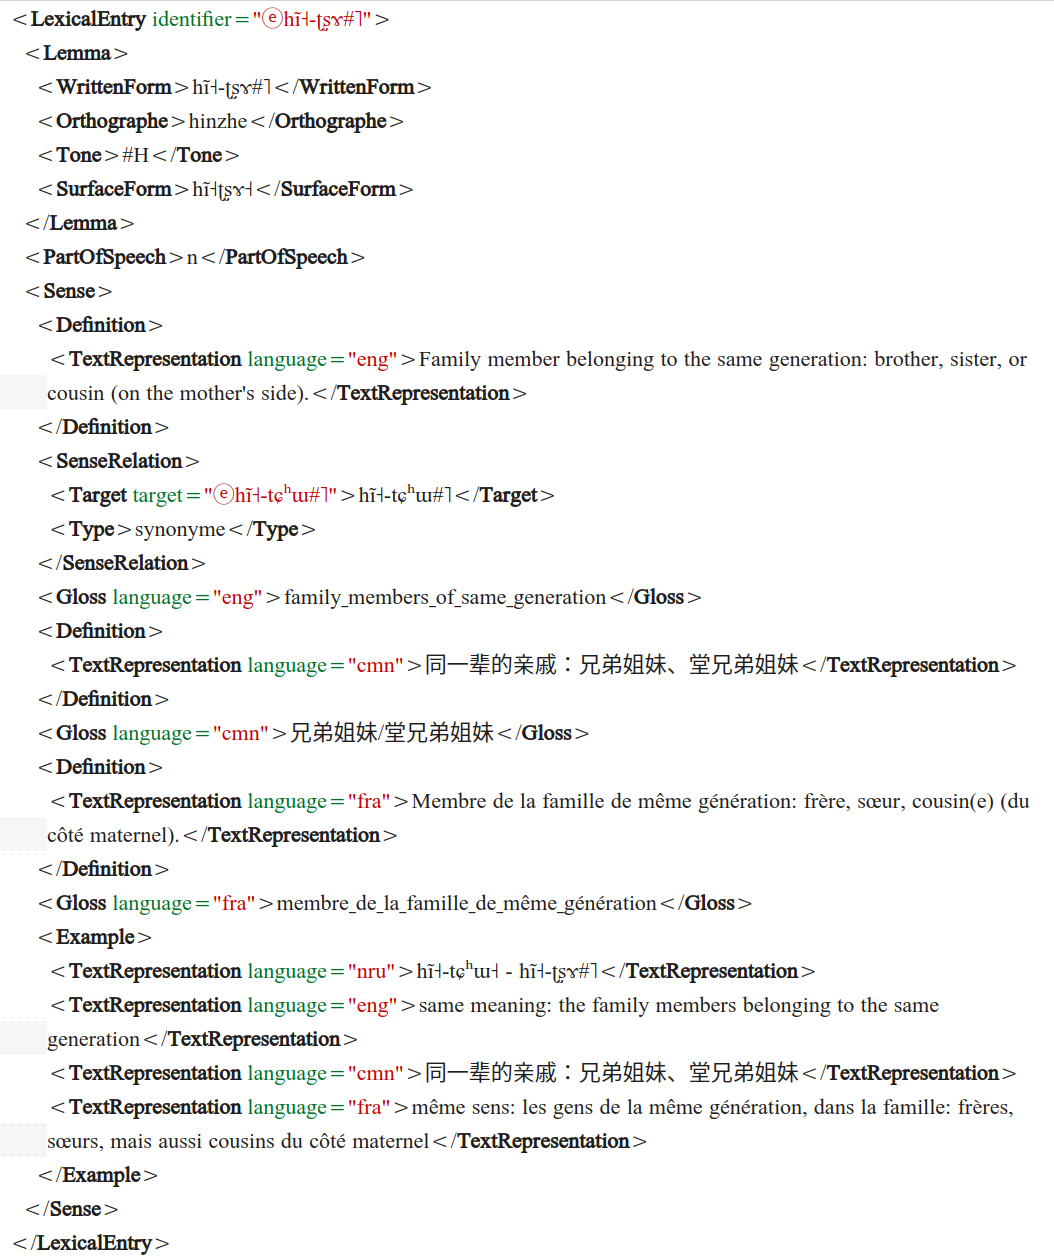
\includegraphics[width=.8\textwidth]{images/LexikaXML.png}
        \caption{A sample entry illustrating the structure of the Lexika XML lexicographic database.}
        \label{fig:LexikaXML}
\end{figure}

The dictionary is made up of \emph{lexical entries}. Each entry has a computer identifier. This identifier is not displayed in the PDF version of the dictionary, as its function is to enable computer manipulation, and not to be recognized by human eyes. This identifier is made up of the special character \textecode{ⓔ} followed by the phonological representation of the word (here, \phonologie{hĩ˧-ʈʂɤ\#˥}), with a tone notation system that uses special symbols (\$ and \#) to distinguish the various kinds of high tones, depending on how they are associated with syllables. Full explanations of this system can be found in the monograph \emph{Tone in Yongning Na}, available online in open access \parencite[80-90]{michaud2017}.

The \emph{lemma} of the lexical entry comprises four pieces of information: its abstract phonological form, its tone, an orthographic representation (provided by Roselle Dobbs), and finally its surface form (which corresponds to its realization when the word is spoken in isolation).

The part of speech (morphosyntactic class) is then provided.

This is followed by a description of the meaning(s) of the word. An indication of the semantic domain is provided, from a closed list of terms (in French and English): ‘society’, ‘house’, ‘body’, ‘plant’, ‘animal’, and so on. This is a rough division, relying partly on form, and partly on semantic contents. No attempt was made to use a fine-grained classification of the sort found in the WordNet database of English, where nouns, verbs, adjectives and adverbs are grouped into sets of cognitive synonyms \parencite{fellbaum2005}.

Definitions are provided in English, Chinese and French. In a few cases, a definition in the vernacular language is provided. The process of producing explanations in the language under study is extremely useful \parencite{dingemanse_folk_2015}, and the co-author of the dictionary is good at it; such definitions nonetheless remain very few to date because too little time was devoted to this task so far.

Glosses are also provided, with a view to future systematic glossing of texts.

The examples are also considered part of the ‘Meaning’ block, insofar as they illustrate one of the meanings of the word. Each example includes a transcription and a translation in the three target languages. Many examples are accompanied by notes, which include an attribute indicating the linguistic field concerned: semantics, syntax, morphology, phonology, tonology,\footnote{(Tonology is coded differently from phonology because of the important role it plays in the documentation and research work carried out)} or dialectology. This additional information appears in the PDF file (unless it carries a print="n" label in the database).

Notes carrying a ‘history’ tag trace the history of notations from the earliest fieldwork to the current version. They provide explanations about the trial-and-error process, the date of adoption of a change in notation, and the arguments in its favour. For instance, the entry \phonologie{ŋwɤ˧pʰæ˧˥} ‘tile' has a note that indicates that it was initially written with a M.H tone pattern, and with a \phonologie{æ} vowel in both syllables: \phonétique{ŋwæ˧pʰæ˥}. The note explains that the perception of \phonétique{æ} in the first syllable is due to a phonetic tendency towards regressive vowel harmony. Verifications are also consigned in this field. About half the entries have information of this type. This sometimes roundabout history did not seem relevant to most readers, so it does not appear in the PDFs.

Semantic relationships such as synonymy are encoded, as is etymology. In the current state of the dictionary, the information somewhat misleadingly labelled as “etymological” essentially consists of synchronic links between a disyllabic or polysyllabic word and the morphemes of which it is (uncontroversially) composed: for example to point out that \phonologie{æ˧ʂæ˧-pi˧mv̩˧˥} 'tale' is formed from the two words \phonologie{æ˧ʂæ\#˥} 'formerly' and \phonologie{pi˧mv̩˥\$} 'saying, adage'.

\subsection{Structure of dictionary entries}
\label{sec:structure_of_entries}

XXXXX FOURNIR ICI UN EXEMPLE

Each entry begins with the headword in phonological transcription -- here, \phonologie{ɑ˩pʰv̩\#˥}. Tone is indicated in terms of phonological categories as analyzed in the monograph \emph{Tone in Yongning Na}, available online in open access \parencite[80-90]{michaud2017}. The International Phonetic Alphabet is supplemented by the special symbols \$ and \#, which are used to distinguish among the various types of High tones, based on their mode of association with syllables.

A surface form is provided to its right, between slanting lines (slashes). It is the surface-phonological form of the word in phonetic alphabet, commonly referred to as the ``citation form''. Tone is indicated in terms of surface tonal realizations. This form (here: \phonétique{ɑ˩pʰv̩˥}) can be read by anyone with a knowledge of the International Phonetic Alphabet, without requiring an understanding of the mapping of underlying phonological tone categories to surface tone in Yongning Na.

For surface-phonological forms, the aim was to achieve greatest simplicity. Special symbols used in the word’s underlying phonological form are removed from the surface form: dashes indicating junctures internal to the word, tilde in reduplicated forms, and the special symbols \$ and \# (used to distinguish among the various types of High tones). For classifiers, the numeral ‘one’ is added before the classifier, because classifiers are not free forms: they cannot be said on their own. For other bound morphemes, such as affixes and clitics, no surface form is indicated.

An orthographic representation is also provided: a notation in a Romanized script devised by Roselle Dobbs and Xióng Yàn \parencite{dobbs_ortho_2018} -- here, \emph{opu}. Orthography was added by Roselle Dobbs, starting in 2017. The transcription was developed with a view to use within the Na community. Importantly, this is not a transliteration of the phonological representation provided in International Phonetic Alphabet. Phonological forms are all based on the dialect of the second author, whereas proposed orthographic representations are intended by Roselle Dobbs, Xiong Yan and their collaborators as a cross-dialect writing system. Given the high degree of dialectal diversity, proposing a transcription that is acceptable for speakers of several dialects implies some compromises. For instance, only the low tone (L) is indicated (with the letter \emph{q} at the end of monosyllabic words), because it was found to be more stable than the other tones across the dialects taken into account when devising the orthography.

Idiolectal similarities and differences in pronunciation are then indicated, by associating the speaker code with the label ‘same’ (if the consultant's pronunciation is identical to that of the co-author of the dictionary, who is the reference speaker) or with an International Phonetic Alphabet transcription of their pronunciation.

The part of speech is indicated using a simple set of labels shown in Table~\ref{table:PartsOfSpeech}.

\begin{longtblr}[
  caption = {Parts of speech},
  label = {table:PartsOfSpeech}
]{
  colspec = {X[l,m]X[l,m]X[l,m]},
  rowhead = 1
}
  \hline
  {abbreviation} & {meaning} & {number of occurrences in dictionary}  \\
  \hline
        \textsc{adj} & adjective & \obtenircompteur{adj} \\
        \textsc{adv} & adverb & \obtenircompteur{adv} \\
        \textsc{clf} & classifier & \obtenircompteur{clf} \\
        \textsc{clitic} & clitic & \obtenircompteur{clitic} \\
        \textsc{cnj} & conjunction & \obtenircompteur{cnj} \\
        \textsc{disc.ptcl} & discourse particle & \obtenircompteur{disc.ptcl} \\
        \textsc{ideophone} & ideophone & \obtenircompteur{ideophone} \\
        \textsc{intj} & interjection & \obtenircompteur{intj} \\
        \textsc{n} & noun & \obtenircompteur{n} \\
        \textsc{num} & numeral & \obtenircompteur{num} \\
        \textsc{postp} & postposition & \obtenircompteur{postp} \\
        \textsc{pref} & prefix & \obtenircompteur{pref} \\
        \textsc{prep} & preposition & \obtenircompteur{prep} \\
        \textsc{pro} & pronoun & \obtenircompteur{pro} \\
        \textsc{suff} & suffix & \obtenircompteur{suff} \\
        \textsc{v} & verb & \obtenircompteur{v} \\
  \hline
\end{longtblr}

The tone category of the word is provided to the right of the part-of-speech label. The tonal class indicated is the underlying phonological category of the word. This information is already present in the phonological transcription, but having it repeated on its own facilitates searches.

Definitions are provided in English, Chinese and French.

Examples fall into three main categories: (i)~``dictionary examples", collected in fieldwork and published specifically as part of the dictionary; (ii)~examples excerpted from the set of Na texts (transcribed audio recordings) in the Pangloss Collection, an open-access online archive \parencite[about which see ][]{michailovskyetal2014}; and (iii)~simple pointers (hyperlinks) to examples in the online archive that appear especially illuminating for the study of the word at issue.

Among examples in set (i), those elicited to study the tones of specific word combinations are preceded by the mention “(Phonological elicitation)”. Proverbs and sayings are marked as “(Proverb)”.

Finally, there are links to related words, such as synonyms, or constituent parts of complex words (labelled as “etymology”, although in view of the shallow temporal depth the label may not be fully deserved). For nouns, the most commonly used classifiers are indicated (here, \phonologie{mi˩}).

Archaic words are singled out as such through the mention “Archaic”.

The dictionary adopts the abbreviations recommended in the Leipzig Glossing Rules \parencite{comrieetal}; all other terms are provided in full. Glosses mostly follow the choices made by \textcite{lidz2010}.

Some monosyllabic roots extracted from disyllables are indicated by the symbol †. No surface form is provided, as these monosyllabic forms are not currently in use in the language.

Borrowings from Chinese and Tibetan are indicated as such in cases where identification seems straightforward. No efforts at systematic elicitation of borrowings from either language were made, but all loanwords occurring in texts were added to the dictionary. The information provided includes: the donor language, the form in the donor language, and occasionally an explanatory note. %When the number of syllables in the borrowed word is the same as in the donor language, the glosses in English (and French) start by the original word followed by two colons and a translation: e.g. ‘\pcmn{办法}::solution’ for \phonologie{pæ˧˥hwɤ˧}.



\subsection{Links to online texts}

As mentioned in §\ref{sec:structure_of_entries}, some of the examples are excerpted from the set of Na texts (transcribed audio recordings) in the Pangloss Collection, an open-access online archive \parencite[about which see ][]{michailovskyetal2014}. A one-click link from the PDF to the exact location of the example in the online archive is offered, by means of the document's Digital Object Identifier (DOI). Simple pointers (a reference and a hyperlink) are also provided for some examples in the online archive that appear especially illuminating for the study of the word at issue, but which it did not seem highly relevant to reproduce in full in the dictionary.

A prospect for future improvement beyond these hand-picked links consists in creating \emph{systematic}, dynamic links between resources, so that dictionaries, primary documentation (the texts that constitute the core of linguistic resources) and grammars can become more and more interconnected \parencite{maxwell2012}. Textual occurrences ultimately constitute the best resource to document a word’s usage. The examples currently presented in the dictionary are few in number, compared to the occurrences in texts, and their context of use may not be clear, despite efforts at providing contextual information for examples jotted down during fieldwork. No time line can be offered as yet concerning the production of complete concordances of occurrences in texts. This development will require glossing the texts at the level of the word and deploying identifiers (such as those used in the lexical database) allowing for error-free mapping from words in texts to dictionary entries.



\section{Lexicology as a research programme}
\label{sec:recherche}

Lexicography has been considered as somewhat peripheral among the language sciences: its task would consist in carrying out a simple inventory. Thus Samuel Johnson, in the Preface to his 1755 \emph{Dictionary of the English Language}, bemoans that

\begin{quotation}
    It is the fate of those who toil at the lower employments of life, to be rather driven by the fear of evil, than attracted by the prospect of good; to be exposed to censure, without hope of praise; to be disgraced by miscarriage, or punished for neglect, where success would have been without applause, and diligence without reward.

    Among these unhappy mortals is the writer of dictionaries; whom mankind have considered, not as the pupil, but the slave of science (...). Every other authour \emph{(sic.)} may aspire to praise; the lexicographer can only hope to escape reproach, and even this negative recompence \emph{(sic.)} has been yet granted to very few.
\end{quotation}

Two and a half centuries later, a professor of linguistics in England provided a pithy summary of the same observation: “the lexicographer is the equivalent in linguistics to the guy stacking the shelves at Sainsbury’s” (anonymized personal communication, 1996). In contrast to the description of the morphosyntax of a language, which aims to highlight the cogency of the grammatical system as a whole, the description of the lexicon tends to be seen as piecemeal in nature. The alphabetical order in which dictionaries are presented looks like a confession that the lexicon lacks internal organization.

This somewhat disparaging view overlooks the many possibilities for developing lexicography into \emph{lexicology}. To write a dictionary is to explore the structure of the lexicon of a language \parencite{francois2008semantic}, in connection with the study of social and cultural structures. Writing a dictionary requires delving into meaning, attempting to delineate connotations, polysemy, and relationships between words. Many dictionary entries could easily be expanded into essays. Thus, the vocabulary of kinship provides valuable insights about family structures and their history. (In the case of the Na language, the usefulness of this source of information has long been recognized \parencite{fu1983}, but it remains to be exploited systematically in light of social dynamics \parencite{milan2021entraide}.) Beyond the semantic domain of kinship (a classic in the field of ethnolinguistic studies), various areas call for exploration, including emotions \parencite{tersis_langage_2017} and spirituality \parencite{francois_shadows_2013}. In-depth lexicographical descriptions can serve as a basis for various research approaches, which combine typology with a dynamic (diachronic) dimension.

One promising strand of research is the study of contact effects on the lexicon.

\begin{quotation}
    “The tendency for bilingual individuals to align the semantic structures of the languages they speak leads to the diffusion of certain lexical categorizations across vast linguistic and cultural areas: thus, specific semantic distinctions, specific patterns of polysemy, specific set phrases become telltale signs of a given area. It is sometimes possible to explain these areal phenomena in terms of links between language use and social practices in the region: certain modes of family organization, for example, may be correlated with specific lexical structures in the field of kinship, or in the vocabulary of marriage and interpersonal relationships.” (Alexandre François \& Lameen Souag, argument of the seminar \emph{« Structures du lexique : typologie et dynamiques »}, LACITO, January 2018)
\end{quotation}

Specifically, comparative research into the lexicon of Na and Pumi \parencite{daudey2014} appears especially promising for an in-depth understanding of the languages and cultures of these two peoples which coexist in the Yongning Plain. This is one of many research issues which it is hoped that the present dictionary will help investigate.

\section*{Acknowledgments}

Many thanks to Picus Ding for putting the first author in touch with the Mosuo scholar Latami Wangyong \pcmn{拉他咪王勇(拉他咪达石)}. Special thanks to Latami Wangyong (and to all family members) for supporting and encouraging our work since 2006. %Many thanks to the main consultant, Latami Dashilame \pcmn{拉它米打史拉么}, and to all family members.

Many thanks to Céline Buret and Séverine Guillaume for engaging in the formatting of the database. Special thanks to Benjamin Galliot for taking charge of computational and typographical matters with loving care since the Autumn of 2016, with an exceptional degree of attention to detail as well as to overall structure. Many thanks to Laurent Romary and Mathieu Mangeot-Nagata for expert advice in digital lexicography, and to Guillaume Jacques for showing the way and for advice along the path.

Many thanks to connoisseurs of the Na culture and language for useful exchanges: Lamu Gatusa \pcmn{拉木·嘎吐萨} (Chinese pen-name: Shi Gaofeng \pcmn{石高峰}), Liberty Lidz, Christine Mathieu, and Pascale-Marie Milan.

Many thanks to Nathan Hill and Tsering Samdrup for identifying names of Tibetan origin. Many thanks to Yi Li \pcmn{衣莉} for suggesting various corrections.

Special thanks to Roselle Dobbs for the flow of information, corrections and advice over the years. Many thanks to Latami Dashi \pcmn{拉他咪王勇(拉他咪达石)} and A Hui \pcmn{阿慧} for suggesting corrections. ``Blessed are the true fault-finders, for they shall be called midwives of truth'' \parencite[vi]{yliniemi_descriptive_2022}. Remaining errors and shortcomings are my own responsibility.

I am grateful to the Dongba Culture Research Institute \pcmn{丽江市东巴文化研究院} in Lijiang for facilitating administrative and practical matters; special thanks to Li Dejing \pcmn{李德静} and to Mu Jihong \pcmn{木霁弘}. At Yunnan University, many thanks are due to Duan Bingchang \pcmn{段炳昌}, Wang Weidong \pcmn{王卫东}, Zhao Yanzhen \pcmn{赵燕珍} and Yang Liquan \pcmn{杨立权} for their careful and sensitive management of fieldwork-related administrative matters.

So many people have supported this project that I must apologize for those names that should be here but were inadvertently left off the list.

This work was supported financially by the ANR project  “Himalayan corpora” (HimalCo, ANR-12-CORP-0006) and by the LabEx “Empirical Foundations of Linguistics” project (EFL, ANR-10-LABX-0083). This work has also benefited from the results of the ANR projects “Phylogenetic assessment of Southern Qiangic” (PASQi, ANR-07-JCJC-0063), “Computational Language Documentation by 2025” (CLD2025, ANR-19-CE38-0015), “Probing neural representations for typological signal” (DeepTypo, ANR-23-CE38-0003) and “Glottalization in the light of Machine Learning” (Glot-TAL, ANR-24-CE38-3766).

I dedicate this work to Juliette Zhao \pcmn{赵筱筠}, my beloved wife.

{\raggedleft Alexis Michaud\par}
